\subsection{Zusammenfassung}

\subsubsection{Mobile Client}
\clearpage

\subsubsection{Entity Relation Diagramm Cloudservice}

\begin{figure}[h]
    \centering
    \begin{minipage}[b]{0.9\textwidth}
        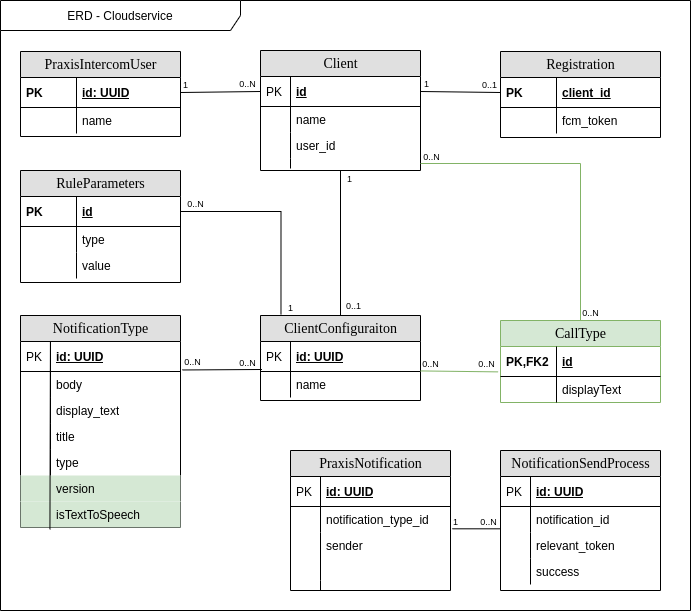
\includegraphics[width=\textwidth]{graphics/diagramms/erd_v02}
        \caption{Entitiy Relation Diagramm - Cloudservice}
    \end{minipage}
\end{figure}

\clearpage
\subsubsection{Klassendiagramm Modul Speech Synthesis}
TODO
\clearpage

\subsubsection{Klassendiagramm Modul Intercom}
TODO
\clearpage

\subsubsection{Schnittstellen Cloudservice}

Der Cloudservice wird um folgende Endpoints erweitert:

\begin{tabularx}{\textwidth}{|p{3cm}|l|l|X|X|}
    \hline
    \textbf{Aktion}                & \textbf{HTTP} & \textbf{Pfad}             & \textbf{Body}   & \textbf{Response} \\
    \hline
    Alle CallTypes laden    & GET          & /api/config/calltype       & - & [CallTypeDto]                 \\
    \hline
    CalLType laden        & GET        & /api/config/calltype/id       & -        & CallTypeDto                 \\
    \hline
    CallType erstellen & POST          & /api/config/calltypes & CallTypeDto & CallTypeDto \\
    \hline
    CallType aktualisieren & PUT          & /api/config/calltypes & CallTypeDto & CallTypeDto \\
    \hline
    CallType löschen & DELETE          & /api/config/calltypes/id & - & - \\
    \hline
    Mehrere CallTypes löschen & DELETE          & /api/config/calltypes/many/filter & - & - \\
    \hline
    Alle CallGroups laden    & GET          & /api/config/callgroup       & - & [CallGroupDto]                 \\
    \hline
    CallGroup laden        & GET        & /api/config/callgroup/id       & -        & CallGroupDto                 \\
    \hline
    CallGroup suchen        & GET        & /api/config/callgroup?callTypeId       & -        & [CallGroupDto]                 \\
    \hline
    CallGroup erstellen & POST          & /api/config/callgroup & CallGroupDto & CallGroupDto \\
    \hline
    CallGroup aktualisieren & PUT          & /api/config/callgroup & CallGroupDto & CallGroupDto \\
    \hline
    CallGroup löschen & DELETE          & /api/config/callgroup/id & - & - \\
    \hline
    Mehrere CallGroups löschen & DELETE          & /api/config/callgroup/many/filter & - & - \\
    \hline
    Sprachsynthese für notificationType        & GET        & /api/speech/id       & -        & MP3 Datei                 \\
    \hline
\end{tabularx}\label{tab:new-api-methods}

Zudem werden die bestehenden Endpoints zur Verwaltung von NotificationType und ClientConfiguration Daten erweitert.
Sodass neu CallTypes auf ClientConfigurations registriert werden können und das isTextToSpeech Flag auf NotificationTypes
gesetzt werden.

Letztlich wird ein neuer Websocket Endpoint unter /api/intercom/signaling veröffentlicht.

\clearpage
